% Created 2025-06-26 Thu 14:45
%& /home/aatmun/.config/emacs/.local/cache/org/persist/55/e635c6-da5d-446d-ac76-e2292edbe935-3d66cee2e73df71d05e76e1f70599acc
% Created 2025-06-26 Thu 14:45
% Intended LaTeX compiler: pdflatex
\documentclass[presentation]{beamer}
\usepackage{amssymb}
\usepackage{hyperref}
\usepackage[utf8]{inputenc}
\usepackage[T1]{fontenc}
\institute{2025 Summer Erdos Institute}

%% ox-latex features:
%   !announce-start, caption, !guess-pollyglossia, !guess-babel, !guess-inputenc,
%   maths, image, !announce-end.

\usepackage{capt-of}

\usepackage{amsmath}
\usepackage{amssymb}

\usepackage{graphicx}

%% end ox-latex features


% end precompiled preamble
\ifcsname endofdump\endcsname\endofdump\fi

\usetheme{Berlin}
\usecolortheme{structure}
\usefonttheme{}
\author{Aatmun Baxi}
\date{}
\title{Quantitative Finance Mini Projects}
\hypersetup{
 pdfauthor={Aatmun Baxi},
 pdftitle={Quantitative Finance Mini Projects},
 pdfkeywords={},
 pdfsubject={},
 pdfcreator={},
 pdflang={English}}
\begin{document}

\maketitle
\begin{frame}[label={sec:orge0092b0}]{Project 1: Risky Portfolio Construction}
\begin{itemize}
\item Focus on \emph{compensated risks} and long term outcomes
\item Invest like someone saving for retirement
\end{itemize}
\pause
\begin{columns}
\begin{column}{0.4\columnwidth}
\begin{block}{Low Risk}
90/10 total mkt stocks/bonds
\pause
\end{block}
\end{column}
\begin{column}{0.6\columnwidth}
\begin{block}{High Risk}
90/10 with Fama-French size \& value factors + Treasury STRIPS
\end{block}
\end{column}
\end{columns}
\end{frame}
\begin{frame}[label={sec:org2cc18f4}]{Results}
\begin{columns}
\end{columns}
\begin{columns}
\begin{column}{0.4\columnwidth}
\begin{block}{Over/Under Performance}
\begin{center}
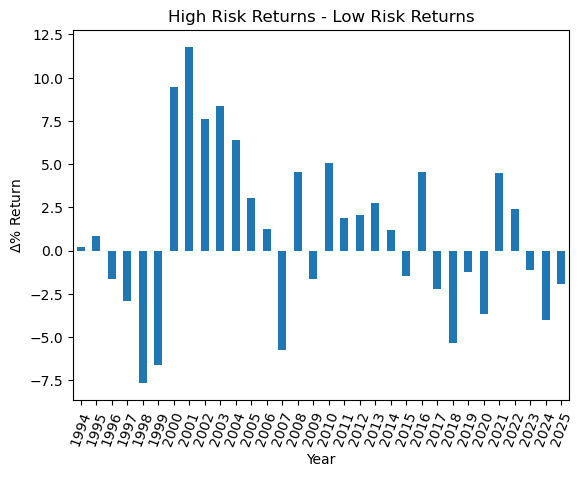
\includegraphics[width=.9\linewidth]{./figures/over-under.png}
\end{center}
\begin{itemize}
\item \tiny{Tracking error introduces behavioral risk}
\end{itemize}
\end{block}
\end{column}
\begin{column}{0.5\columnwidth}
\begin{block}{Backtest}
\begin{center}
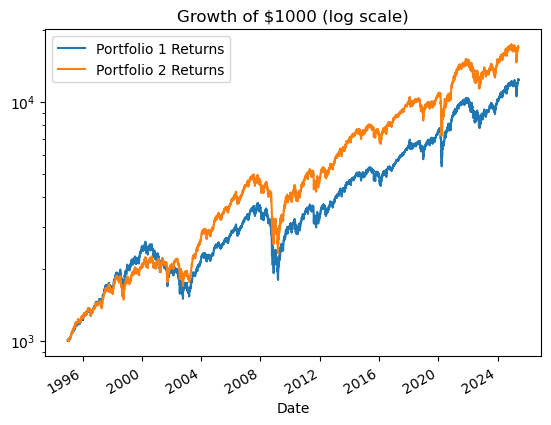
\includegraphics[width=0.8\textwidth]{./figures/backtest.png}
\end{center}


\begin{itemize}
\item \tiny{Low risk \(\sigma =0.159\)}
\item \tiny{High risk \(\sigma =0.155\)}
\item \tiny{Traditional risk metrics largely unchanged!}
\end{itemize}
\vspace{0.5}
\end{block}
\end{column}
\end{columns}
\end{frame}
\begin{frame}[label={sec:orgb67c8a8}]{Project 2: Assumptions of Lognormal Returns}
\begin{itemize}
\item Lognormal daily returns are \alert{very rare} over contiguous periods of time
\begin{itemize}
\item Like a coin flip over rolling 6 month periods
\end{itemize}
\item Hypothesis testing unreliable with large samples
\end{itemize}

\begin{figure}[htbp]
\centering
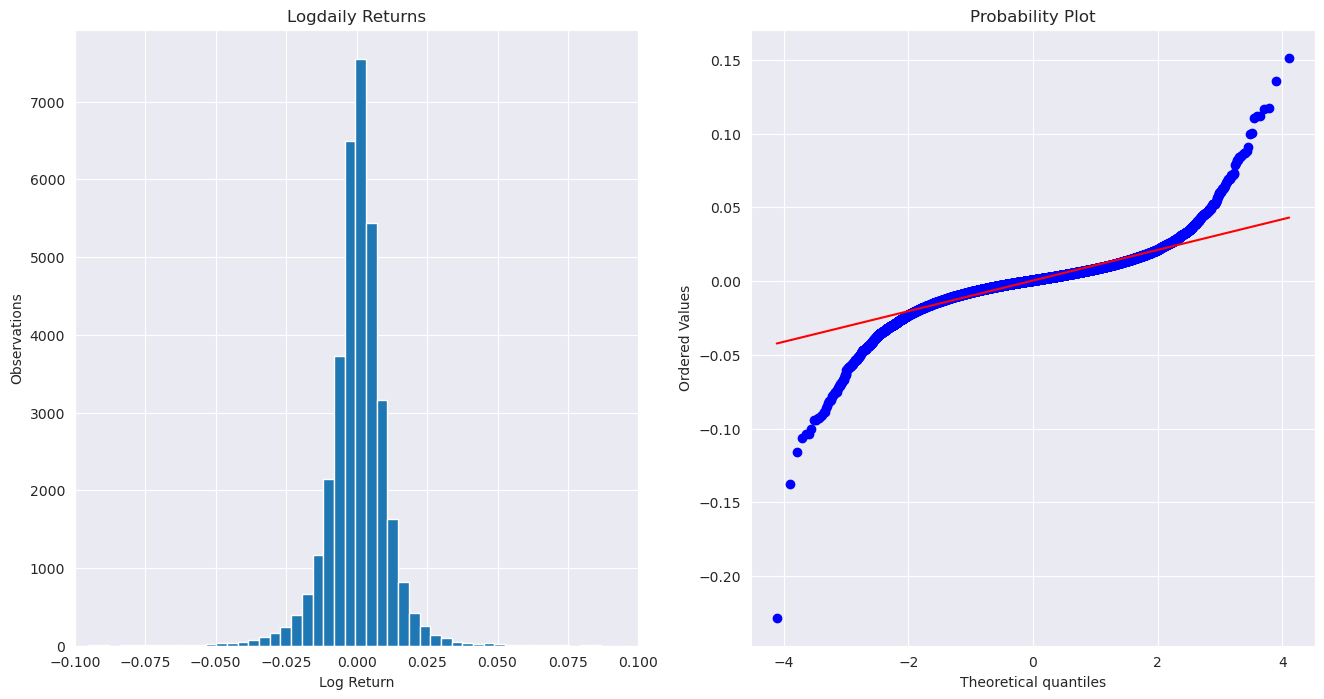
\includegraphics[width=0.7\textwidth]{./figures/sp500-probplots.png}
\caption{S\&P 500 Log Returns}
\end{figure}
\end{frame}
\begin{frame}[label={sec:org5db85f6}]{Local Behavior of Log Returns}
\begin{figure}[htbp]
\centering
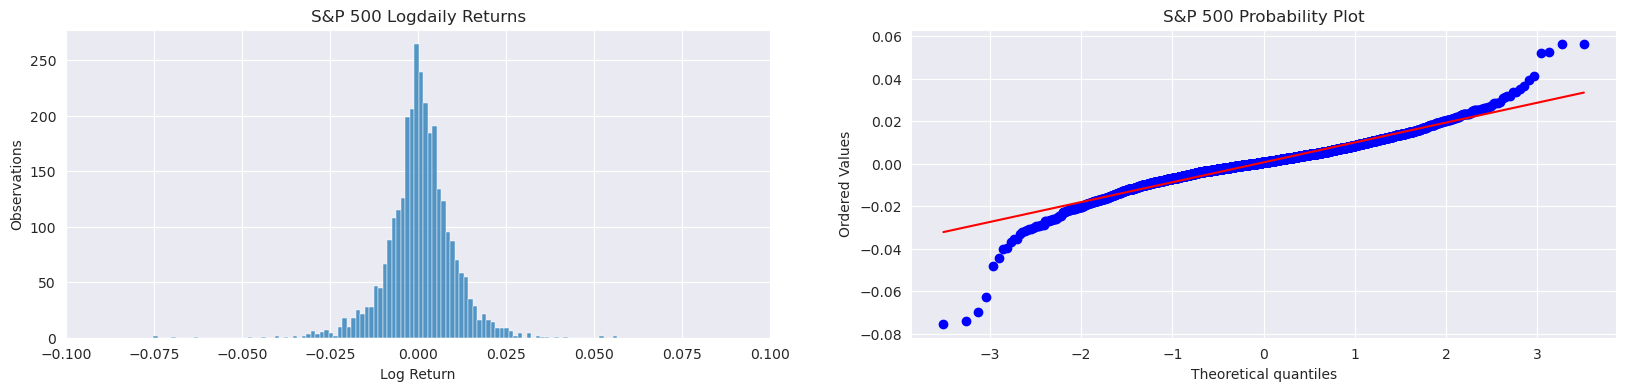
\includegraphics[width=\textwidth,height=3.5cm]{./figures/sp500-bull-probplot.png}
\caption{S\&P 500 Log Returns: 1987/12 to 2000/03}
\end{figure}
\end{frame}
\begin{frame}[label={sec:org056754f}]{Local Behavior of Individual Stock Log Returns}
\begin{figure}[htbp]
\centering
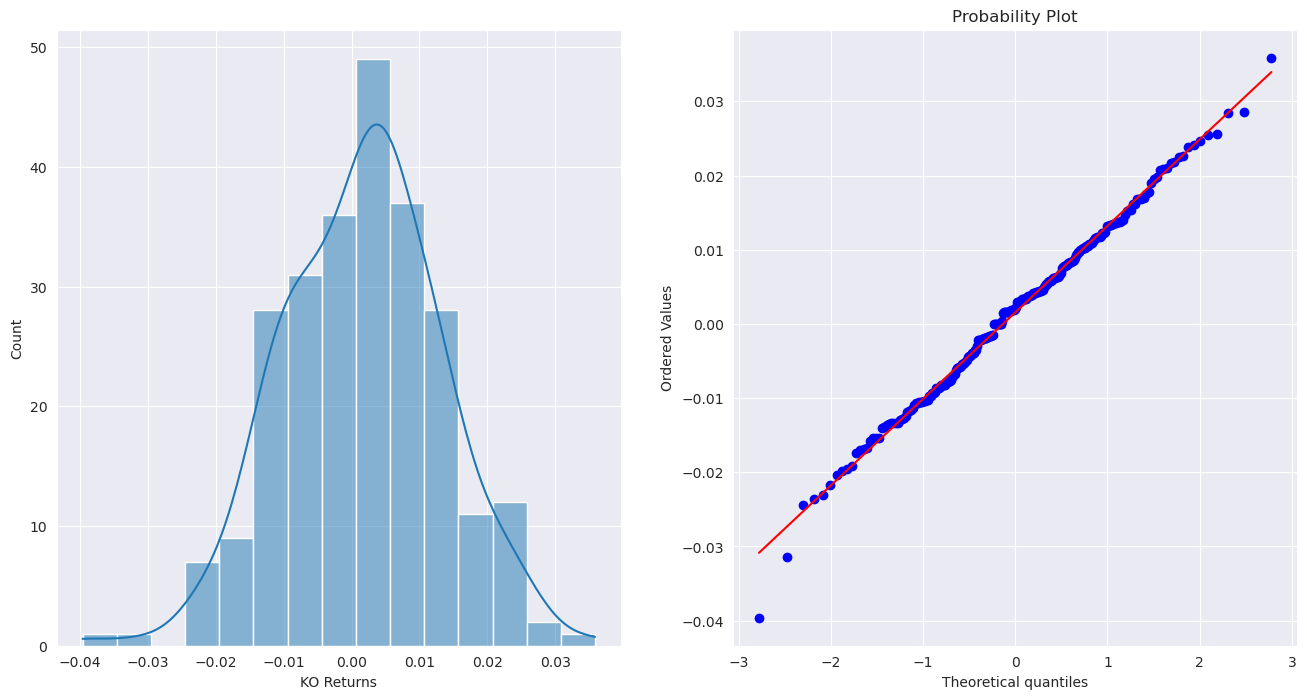
\includegraphics[width=.9\linewidth]{./figures/ko-normal.png}
\caption{KO Log Returns: 1995/04 to 1996/04}
\end{figure}
\end{frame}
\begin{frame}[label={sec:org5184bb1}]{Project 3: TTE and Spot Dependence of BS Option Prices}
\begin{itemize}
\item Discovered \alert{theta decay} and options as \alert{leveraged long/short positions}
\end{itemize}
\begin{columns}
\begin{column}{0.5\columnwidth}
\begin{figure}[htbp]
\centering
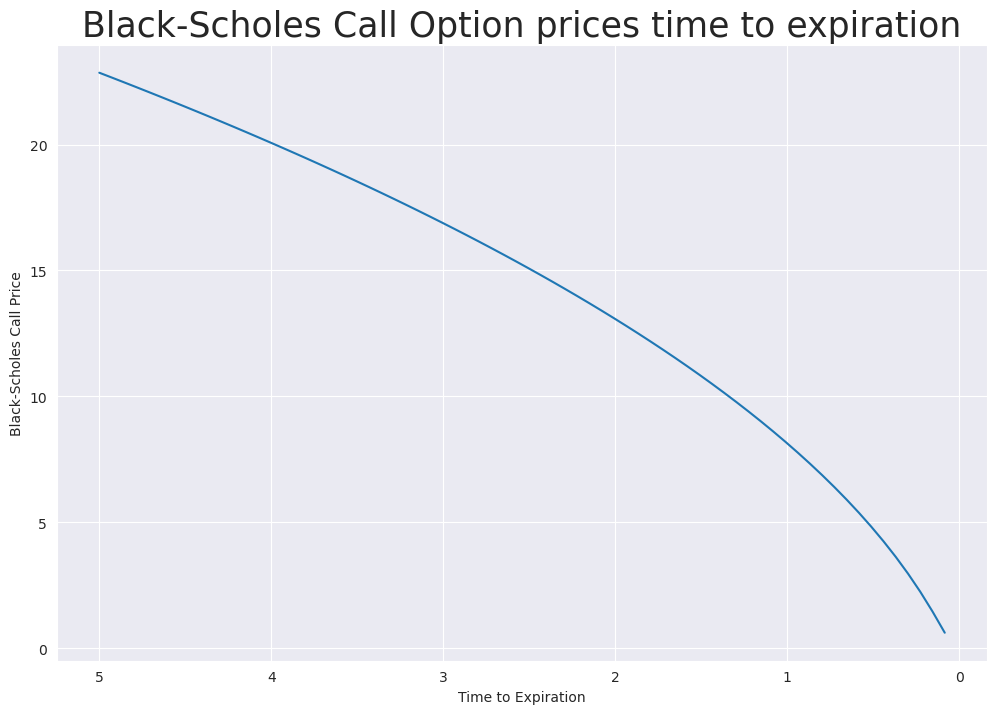
\includegraphics[width=.9\linewidth]{./figures/bc-call-tte.png}
\caption{\$110C @ \$100 spot. Time to Expiration Dependence}
\end{figure}
\end{column}
\begin{column}{0.5\columnwidth}
\begin{figure}[htbp]
\centering
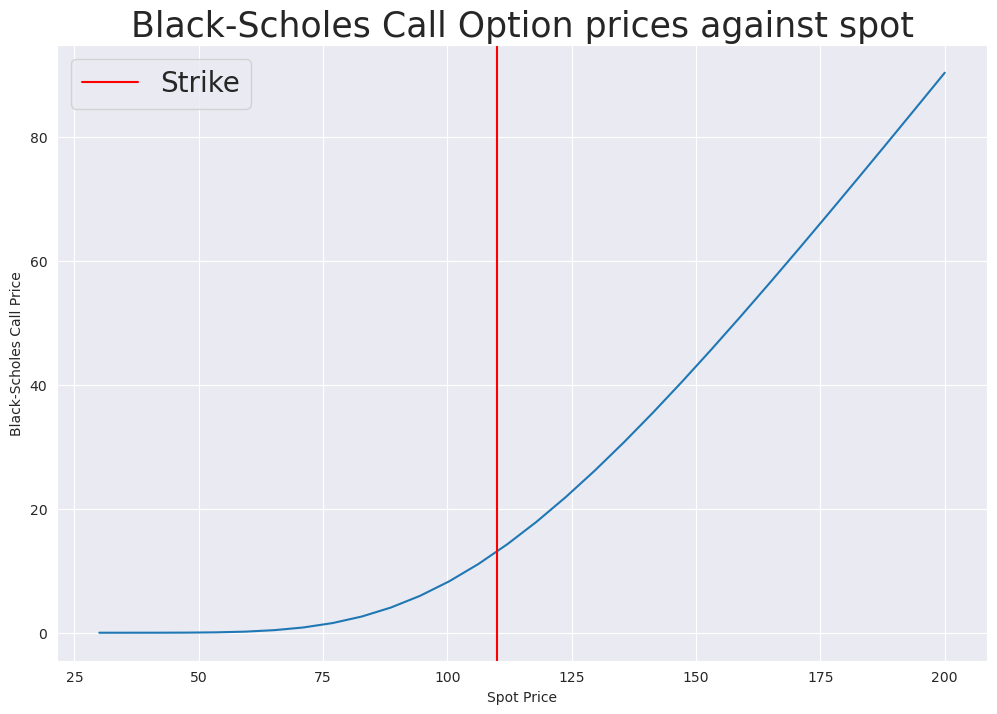
\includegraphics[width=.9\linewidth]{./figures/bc-call-spot.png}
\caption{\$110C @ \$100 spot. Spot Dependence}
\end{figure}
\end{column}
\end{columns}
\end{frame}
\begin{frame}[label={sec:orge5b486e}]{Phenomena in Context of Trading Strategies}
\begin{itemize}
\item Theta decay: a double edged sword
\begin{itemize}
\item \alert{Hurts} option buyers
\item \alert{Helps} option sellers
\item Covered calls/puts exploit this theta decay
\item Justifies multi-leg strategies to protect against losses
\end{itemize}
\end{itemize}


\begin{itemize}
\item Deep ITM options as leveraged  positions
\begin{itemize}
\item \(|\Delta |\) values close to \(1\) give near equivalent directional exposure to 100x the underlying
\item Theta decay reduced at long expirys, ergo\ldots{}
\item Deep ITM LEAPS get best of \(\Delta\) exposure and least theta decay
\end{itemize}
\end{itemize}
\end{frame}
\begin{frame}[label={sec:org04b22c4}]{Project 4: Effects of Volatility Models on \(\Delta\) Hedging}
\begin{block}{Main Accomplishment}
\begin{itemize}
\item Implemented \alert{generic Monte Carlo method} for both options pricing and delta approximation
\item Allowed for a fully simulated \(\Delta\) hedging payoff model
\item Plug-and-play with various stochastic processes
\end{itemize}
\pause
\end{block}
\begin{block}{Models tested}
Constant volatility, constant elasticity of variance (CEV), Hull-White stochastic vol, GARCH(1,1), SABR
\end{block}
\end{frame}
\begin{frame}[label={sec:orgfad2c70}]{Some Profit Distributions}
\begin{columns}
\begin{column}{0.5\columnwidth}
\begin{figure}[htbp]
\centering
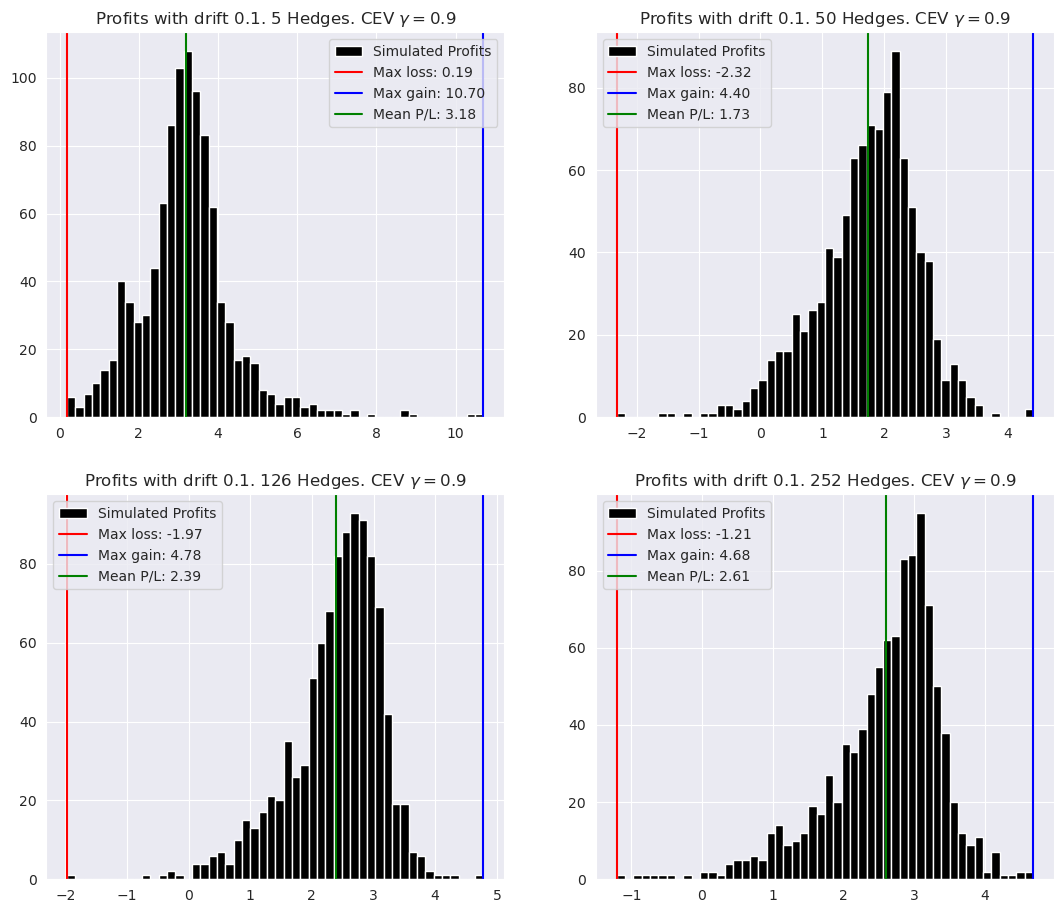
\includegraphics[width=.9\linewidth]{./figures/cev-distribution.png}
\caption{CEV Profit Distributions}
\end{figure}
\end{column}
\begin{column}{0.5\columnwidth}
\begin{figure}[htbp]
\centering
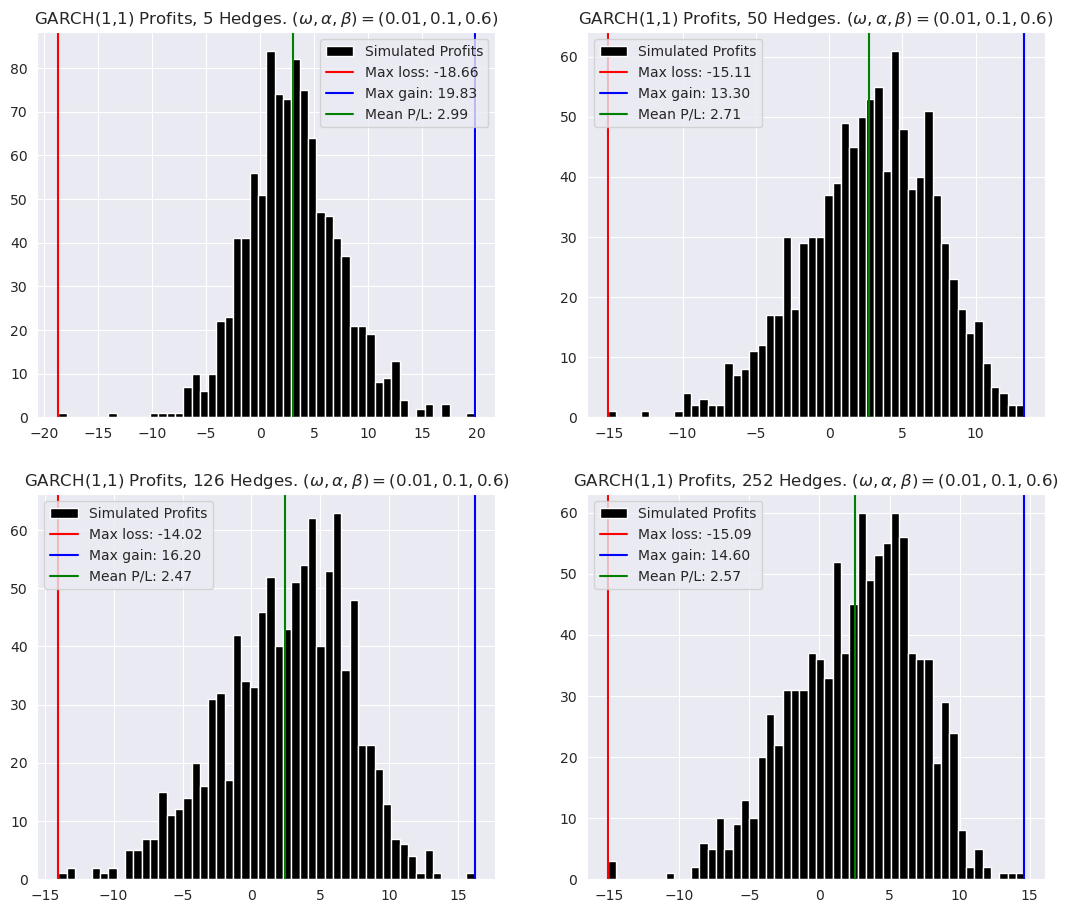
\includegraphics[width=.9\linewidth]{./figures/GARCH-distribution.png}
\caption{GARCH(1,1) Profit Distributions}
\end{figure}
\end{column}
\end{columns}
\end{frame}
\begin{frame}[label={sec:org9419282}]{Conclusion}
Thank you for your attention!
\end{frame}
\end{document}
